\chapter{Охрана труда и экология}
\label{cha:ecolog}

\section{Анализ опасных и вредных факторов при использовании программного
	обеспечения и мероприятия по их устранению}
Процесс создания и использования программного обеспечения невозможен без использования
персональных электронно-вычислительных машин (ПЭВМ). Эксплуатация ПЭВМ
сопряжена с рядом вредных факторов, воздействию котрых подвергаются
пользователи. К таким факторам относятся электромагнитное излучение,
отраженный свет и блики, вибрация, шум.

В данном разделе рассматриваются основные виды опасных и вредных факторов, а
также допустимые нормы излучений, требования к освещенности, помещению в
целом, уровням шума на рабочем месте, которые регламентируются СанПиН
2.2.2/2.4.1340-03 <<Гигиенические требования к персональным
электронно-вычислительным машинам и организация рабочего места>>

\subsection{Требования к помещению для работы с ПЭВМ}
Обучение и работа с ПЭВМ должны проходить в помещении, которое не наносит
вреда здоровью и создает комфортные условия труда. Следует придерживаться
общих рекомендаций при выборе помещения и материалов для его внутренней
отделки:
\begin{enumerate}
\item Окна в помещениях, где используется вычислительная техника,
	преимущественно должны быть ориентированы на север и северо-восток.
	Оконные проемы должны быть оборудованы регулируемыми устройствами
	типа: жалюзи, занавесей, внешних козырьков и т.д.

\item Для внутренней отделки интерьера помещений, где расположены ПЭВМ, должны
	использоваться диффузно отражающие материалы с коэффициентом отражения
	для потолка: $0.7 - 0.8$; для стен: $0.5 - 0.6$; для потолка: $0.3 -
	0.5$.
\item Помещения, где размещаются рабочие места с ПЭВМ, должны быть оборудованы
	защитным заземлением в соответствии с техническими требования по
	эксплуатации.
\item Не следует размещать рабочие места с ПЭВМ вблизи силовых кабелей и
	вводов, высоковольтных транформаторов, технологического оборудования,
	создающего помехи в работе ПЭВМ.
\end{enumerate}

\subsection{Общие требования к организации рабочих мест пользователей ПЭВМ}
Пользователи ПЭВМ в первую очередь подвержены воздействию излучения от экрана
мониторов, поэтому экран видеомонитора должен находиться на расстоянии $600 -
700$~мм от глаз пользователя, но не ближе 500~мм с учетом размеров
алфавитно-цифровых знаков и символов.

Для комфортной организации рабочих мест расстояние между рабочими столами с
видеомониторами должно быть не менее 2.0~м, а расстояние между боковыми
поверхностями видеомониторов -- не менее 1.2~м. СанПиН 2.2.2/2.4.1340-03
рекомендует изолировать рабочие места друг от друга перегородками высотой $1.5
- 2.0$~м. Для снижения утомляемости пользователей рабочее кресло должно быть
подъемно-поворотным, регулируемым по высоте и по углам наклона сиденья и
спинки, а также расстоянию спинки от переднего края сиденья.

\subsection{Требования к микроклимату}
Процесс написания/изучения работы программного продукта требует повышенной
концентрации внимания, умственных усилий, что сопровождается
неврно-эмоциональным напряжением. Данный вид работ относится к категории 1а.
Такие помещения согласно СанПиН должны обеспечиваться оптимальными параметрами
микроклимата. Оптимальные параметры микроклимата указаны в
таблице~\ref{tab:optimal_microclimat}.

\begin{table}[ht!]
  \centering
  \caption{Оптимальные параметры микроклимата}
  \label{tab:optimal_microclimat}

  \begin{tabular}{|c|c|c|c|}
    \hline
    \thead{Период года} & \thead{Температура \\ воздуха, \celsius} & \thead{Относительная \\ влажность воздуха, \%} &
    \thead{Скорость движения воздуха, м/c \\ (не более)} \\
    \hline
    Холодный   & 22-24 & 40-60 & 0.1 \\
    \hline
    Теплый   & 23-25 & 40-60 &  0.1 \\
    \hline
  \end{tabular}
\end{table}

К вредным факторам при работе с ЭВМ относят также и запыленность помещения.
Этот фактор усугубляется влиянием электростатических полей персональных
компьютеров. Необходимо производить влажную уборку и проветривать помещение.

\subsection{Требования к уровню шума и вибрации}
Уровень шума на рабочем месте не должен превышать 50~дБA, а уровни вибрации не
должны превышать предельно допустимых значений, указанных в
таблице~\ref{tab:vibration}.

\begin{table}[ht!]
  \centering
  \caption{Допустимые нормы вибрации на рабочих местах с ПЭВМ}
  \label{tab:vibration}
  \begin{tabular}{|p{0.35\textwidth}|p{0.20\textwidth}|p{0.20\textwidth}|}
    \hline
    \multirow{2}{\hsize}{Среднегеометрические частоты октавных полос, Гц} &
    \multicolumn{2}{|c|}{Допустимые значения по виброскорости} \\
    \cline{2-3}
    & м/с & дБ \\
    \hline
    2 & 45 & 79 \\
    \hline
    4 & 22 & 73 \\
    \hline
    8 & 11 & 67\\
    \hline
    16 & 11 & 67 \\
    \hline
    31.5 & 11 & 67 \\
    \hline
    63 & 11 & 67 \\
    \hline
    Корректированные значения и их уровни в дБ & 20 & 72 \\
    \hline
  \end{tabular}
\end{table}

К внутренним источникам шума относятся вентиляторы, принтеры и другие
периферийные устройства ЭВМ.

Мощные источники шума, такие как сервера должны быть расположены в отдельных
помещениях с использованием средств звукоизоляции (звукопоглощающих материалов
для облицовки стен и потолка помещения) и толстых перегородок (стен).

К внешним источникам шума можно отнести шум с улицы и соседних помещений. Для
снижения шума улицы следует использовать более толстые шумопоглощающие
стеклопакеты. Для уменьшения шума соседних комнат следует использовать облицовку
стен звукопоглощающими материалами.

\subsection{Требования к освещенности}
Наиболее важным условием эффективной работы пользователей является соблюдение
оптимальных параметров системы освещения в рабочих помещениях.

В соответствии с СанПиН 2.2.2/2.4.1340-03 освещенность на поверхности рабочего
стола должна находиться в пределах 300-500~лк. Разрешается использование
светильников местного освещения для работы с документами (при этом светильники
не должны создвать блики на поверхности экрана).

Правильное расположение рабочих мест относительно источников освещения,
отсутствие зеркальных поверхностей и использование матовых материалов
ограничивает прямую (от источников освещения) и отраженную (от рабочих
поверхностей) блескость. При этом яркость светящихся поверхностей и потолка не превышает
$200~\textup{кд}/\textup{м}^{2}$, яркость бликов на экране ПЭВМ не превышает
$40~\textup{кд}/\textup{м}^{2}$.

\subsection{Требования к уровням электромагнитных полей на рабочих местах,
оборудованных ПЭВМ}
При использовании ПЭВМ пользователи подвергаются воздействию электромагнитного
излучения. Уровни электромагнитных полей нормируются по СанПиН
2.2.2/2.4.1340-03 и представлены в таблице~\ref{tab:vdu_emp} и
таблице~\ref{tab:visual_vdt}.

\begin{table}[ht!]
  \centering
  \caption{Временные допустимые уровни ЭМП, создаваемых ПЭВМ}
  \label{tab:vdu_emp}
  \begin{tabular}{|p{0.22\textwidth}|p{0.37\textwidth}|p{0.20\textwidth}|}
    \hline
    \multicolumn{2}{|c|}{Наименование параметров} & ВДУ ЭМП \\
    \hline
    \multirow{2}{\hsize}{Напряженность электрического поля}
        & в диапазоне частот 5~Гц - 2~кГц & 25~В/м\\
        \cline{2-3}
        & в диапазоне частот 2~кГц - 400~кГц & 2.5~В/м\\
    \hline
    \multirow{2}{\hsize}{Плотность магнитного потока}
        & в диапазоне частот 5~Гц - 2~кГц & 250~нТл\\
        \cline{2-3}
        & в диапазоне частот 2~кГц - 400~кГц & 25~нТл\\
    \hline
    \multicolumn{2}{|c|}{Электростатический потенциал экрана видеомонитора} & 500~В \\
    \hline
  \end{tabular}
\end{table}

\begin{table}[ht!]
  \centering
  \caption{Визуальные параметры ВДТ, контролируемые на рабочих местах}
  \label{tab:visual_vdt}
  \begin{tabular}{|p{0.45\textwidth}|p{0.45\textwidth}|}
    \hline
    Параметры & Допустимы значения \\
    \hline
    Яркость белого поля & Не менее $ 35~\textup{кд}/\textup{м}^{2}$ \\
    \hline
    Неравномерность яркости рабочего поля & Не более $\pm 20\% $ \\
    \hline
    Контрастность (для монохромного режима) & Не менее 3:1\\
    \hline
    Временная нестабильность изображения (мелькания) & Не должна фиксироваться \\
    \hline
  \end{tabular}
\end{table}


\section{Расчет вентиляции}
Расчеты воздухообмена в системах общеобменной и смешанной вентиляции рекомендуется проводить
по следующим показателям~\cite{ventilation}: нормируемой кратности воздухообмена, нормируемому
удельному расходу приточного воздуха, интенсивности вредных выделений, к которым относятся
избытки явной теплоты, избытки влаги и вредные вещества. При этом вычисления следует выполнять
как для теплого, так и для холодного времени года. За конечный результат принимают большее
значение из полученных расчетами по перечисленным выше показателям.

Рассмотрим компьютерный класс со следующими характеристиками:
\begin{enumerate}
\item Количество мест: 30
\item Длинна: 15~м
\item Ширина: 9~м
\item Высота: 5~м
\end{enumerate}

\subsection{Расчет воздухообмена по удельному расходу приточного воздуха}
Расчет по нормируемому удельному расходу приточного воздуха выполняют по формулам
\begin{equation}
	L_{m} = mN,
\label{equ:ventilation_in}
\end{equation}

где $m$ -- нормируемый расход приточного воздуха $\textup{м}^{3}/\textup{ч}$, на одного человека,
одно рабочее место, единицу оборудования; $N$ -- число людей, рабочих мест, единиц оборудования.

Согласно ~\cite{ventilation}, $m = 20~\textup{м}^{3}/\textup{ч}$.
Таким образом требуемый воздухообмен составляет: $20 \cdot 30 = 600~\textup{м}^{3}/\textup{ч}$.

\subsection{Расчет по интенсивности вредных выделений}
Рассмотрим систему механической вентиляции помещения (рис.~\ref{fig:ventilation}).
В общем случае она содержит приточную вентиляцию, подающую воздух в помещение с
массовым расходом $G_{\textup{пр}}$ и вытяжную вентиляцию, удаляющую воздух из верхней
и рабочей зон помещения с массовыми расходами соответственно $G_{\textup{вз}}$ и $G_{\textup{рз}}$.
При этом из рабочей зоны воздух может удаляться как общеобменной вентиляцией, так и местными
отсосами. Вентиляция должна обеспечивать удаление избытков теплоты, влаги и вредных веществ.

\begin{figure}[ht!]
  \centering
  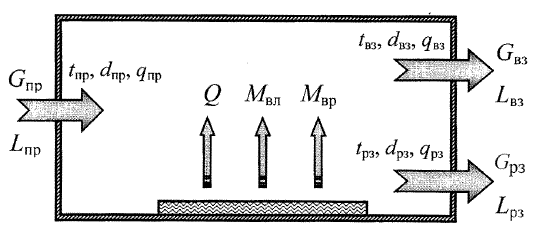
\includegraphics[width=0.5\textwidth]{inc/png/ventilation.png}
  \caption{Схема воздухообмена в помещении}
  \label{fig:ventilation}
\end{figure}

Балансы явной теплоты и воздуха в помещении описываются следующей системой уравнений:
\begin{equation}
	3.6Q + G_{\textup{пр}}c_{p}t_{\textup{пр}} - G_{\textup{вз}}c_{p}t_{\textup{вз}} - G_{\textup{рз}}c_{p}t_{\textup{рз}} = 0;
\label{equ:heat_balance}
\end{equation}
\begin{equation}
	G_{\textup{пр}} - G_{\textup{вз}} - G_{\textup{рз}} = 0,
\label{equ:air_balance}
\end{equation}

где $Q$ -- избытки явной теплоты в помещении, Вт; $c_{p}$ -- удельная теплоемкость воздуха;
$c_{p} \approx 1.0~\textup{кДж}/(\textup{кг} \cdot \celsius)$;
$t_{\textup{пр}},t_{\textup{вз}},t_{\textup{рз}}$ -- температуры соответственно приточного воздуха,
воздуха в верхней и рабочей зонах помещения, \celsius. Обратимся к первому слагаемому в уравнении~\ref{equ:heat_balance},
введя для него обозначение $Q' = 3.6Q$. Так же, как и все остальные слагаемые в этом уравнении, оно имеет размерность~кДж/ч.
Отсюда получим следующее выражение для массового расхода воздуха, удаляемого из верхней зоны:
\begin{equation}
	G_{\textup{вз}} = \frac{Q' - G_{\textup{рз}}c_{p}(t_{\textup{рз}} - t_{\textup{пр}})}{c_{p}(t_{\textup{вз}} - t_{\textup{пр}})}.
\label{equ:top_area_mass_consumption}
\end{equation}

Перейдем в формулах (\ref{equ:air_balance}), (\ref{equ:top_area_mass_consumption}) от массовых расходов к объемным с помощью соотношений
$L_{\textup{пр}} = G_{\textup{пр}} / \rho_{\textup{пр}},
 L_{\textup{вз}} = G_{\textup{вз}} / \rho_{\textup{вз}},
 L_{\textup{рз}} = G_{\textup{рз}} / \rho_{\textup{рз}}$, где $\rho_{\textup{пр}}, \rho_{\textup{вз}}, \rho_{\textup{рз}}$
-- плотности соответственно приточного воздуха и воздуха в верхней и рабочей зонах помещения, $\textup{кг}/\textup{м}^{3}$. В результате получим
\begin{equation}
	L_{\textup{вз}} = \frac{Q' - L_{\textup{рз}}\rho_{\textup{рз}}c_{p}(t_{\textup{рз}} - t_{\textup{пр}})}{\rho_{\textup{вз}}c_{p}(t_{\textup{вз}} - t_{\textup{пр}})}.
\label{equ:top_area_volume_consumption}
\end{equation}
\begin{equation}
	L_{\textup{пр}} = L_{\textup{вз}}\rho_{\textup{вз}}/\rho_{\textup{пр}} + L_{\textup{рз}}\rho_{\textup{рз}}/\rho_{\textup{пр}}.
\label{equ:air_volume_balance}
\end{equation}

Температуру наружного воздуха,~\celsius, для теплого периода года
определяют параметрами А, а для холодного периода года -- параметрами Б (таблица~\ref{tab:temperature_params}).

\begin{table}[ht!]
  \centering
  \caption{Расчетные значения параметров наружного воздуха для Москвы по СП~131.13330-2012}
  \label{tab:temperature_params}
  \begin{tabular}{|c|c|c|c|c|c|c|}
    \hline
    \thead{Период \\ года} & \thead{Параметры} & \thead{Температура \\ воздуха, \\ \celsius} &
	\thead{Удельная \\ энтальпия, \\ кДж/кг} & \thead{Скорость \\ ветра, м/~\\c} &
	\thead{Средне- \\ суточная \\ амплитуда \\ температуры, \\ \celsius} & \thead{Баромет- \\ рическое \\ давление, \\ кПа} \\
    \hline
    \multirow{2}{*}{Теплый} & A & 22.3 & 49.4 & 1 & 10.4 & 99 \\
    \cline{2-7}
                            & Б & 28.5 & 54 & 1 & 10.4 & 99 \\
    \hline
    \multirow{2}{*}{Холодный} & A & -15 & -11.4 & 4.7 & - & 99 \\
    \cline{2-7}
                              & Б & -26 & -25.3 & 4 & - & 99 \\
    \hline
  \end{tabular}
\end{table}

Температура воздуха $t_{\textup{вз}}$, удаляемого из верхней зоны помещения,
зависит от многих факторов, в частности от особенностей организации воздухообмена в помещении. В некоторых
случаях для помещения высотой более 4~м она может быть расчитана по формуле
\begin{equation}
	t_{\textup{вз}} = t_{\textup{рз}} + \Delta(H - 2),
\label{equ:temp_top_zone}
\end{equation}

где $\Delta$ -- градиент температуры по высоте помещения, \celsius/м, зависящий от особенностей теплообмена
в помещении и определяемый, как правило, по результатам натурных измерений; $H$ -- расстояние от пола до
центра вытяжных отверстий в помещении, м. При этом для помещений с незначительными избытками теплоты,
не превышающими $23~\textup{Вт}/\textup{м}^{3}$, полагают $\Delta = 0.2...0.5~\celsius/\textup{м}$; при
значительных избытках теплоты в помещении, превышающих $23~\textup{Вт}/\textup{м}^{3}$, полагают
$\Delta = 0.7...1.5~\celsius/\textup{м}$. Следует отметить, что приведенные значения $\Delta$ применимы только
для схемы воздухообмена <<снизу-вверх>>, т.е. при подаче приточного воздуха в рабочую зону помещения и удалении
нагретого воздуха из верхней зоны. Когда приточный воздух подается в верхнюю зону, значение температурного градиента
будет близко к нулю, так что $t_{\textup{вз}} \approx t_{\textup{рз}}$.

Если значения температуры приточного воздуха и воздуха в помещении отличаются не более чем на 15~\celsius,
то с погрешностью, не превышаюшей 5\%, можно положить $\rho_{\textup{пр}} = \rho_{\textup{вз}} = \rho_{\textup{рз}}$.
При этом уравнения (\ref{equ:top_area_volume_consumption}), (\ref{equ:air_volume_balance}) примут вид
\begin{equation}
	L_{\textup{вз}} = \frac{Q' - L_{\textup{рз}}\rho_{\textup{пр}}c_{p}(t_{\textup{рз}} - t_{\textup{пр}})}{\rho_{\textup{пр}}c_{p}(t_{\textup{вз}} - t_{\textup{пр}})};
\label{equ:top_area_volume_consumption_simple}
\end{equation}
\begin{equation}
	L_{\textup{пр}} = L_{\textup{вз}} + L_{\textup{рз}}.
\label{equ:air_volume_balance_simple}
\end{equation}

Средняя потребляемая мощность ПК составляет 350~Вт, будем считать что $1/3$ переходит в теплоту,
тепловыделения от одного человека составляют 100~Вт таким образом избыток теплоты составляет
$30 \cdot 350/3 + 30 \cdot 100 = 6500$~Вт = 6.5~кВт.

Будем считать, что воздух удаляется только из верхней зоны, т.е. $L_{\textup{рз}} = 0~\textup{м}^{3}/\textup{ч}$.

Для теплого периода года температура наружного воздуха, соответствующая параметрам А (таблица~\ref{tab:temperature_params}),
равна 22.3~\celsius, для холодного -- -26~\celsius (параметры Б).

Определим теперь удельные избытки теплоты в помещении. Для этого вычислим сначала объем помещения
$V = 15 \cdot 9 \cdot 5 = 675~\textup{м}^{3}$. Удельные избытки теплоты $q = 6500 / 675 \approx 10~\textup{Вт}/\textup{м}^3$,
что меньше $23~\textup{Вт}/\textup{м}^3$. Поэтому они являются незначительными.

Положим, что приточный воздух подается в рабочую зону. Тогда температуру в верхней зоне помещений можно определить по
формуле (\ref{equ:temp_top_zone}), приняв $\Delta = 0.5~\celsius/\textup{м}$. Полагая также, что центр вытяжных отверстий располагается на
высоте 4.5~м от пола, находим что температура воздуха в верхней зоне
$t_{\textup{вз.тепл}} = 25 + 0.5(4.5-2) = 26.25~\celsius$ и $t_{\textup{вз.хол}} = 24 + 0.5(4.5-2) = 25.25~\celsius$.

Теперь можно определить расход воздуха в верхней зоне. Согласно (\ref{equ:top_area_volume_consumption_simple}) будем иметь
$L_{\textup{пр.тепл}} = \frac{3.6 \cdot 6500}{1.2 \cdot 1.0 (26.25 - 22.3)} \approx 4937~\textup{м}^{3}/\textup{ч}.$ и
$L_{\textup{пр.хол}} = \frac{3.6 \cdot 6500}{1.2 \cdot 1.0 (25.25 - -26)} = 380.49~\textup{м}^{3}/\textup{ч}.$

Таким образом требуемый воздухообмен составляет $5000~\textup{м}^{3}/\textup{ч}$.

В слишком теплые дни вентиляция будет только ухудшать ситуацию и тогда необходимо использовать кондиционер.

\section{Утилизация пластмасс, являющихся частью жидко-кристаллического монитора}
Процесс переработки начинается с ручного демонтажа составных частей электронной техники.
Демонтированные компоненты, как правило, сортируются на пластик, металл, печатные платы,
провода, люминесцентные лампы, ЖК-дисплеи для дальнейшей переработки.
В данной главе будет рассмотрен процесс утилизации пластика.

Пластмассы — это материалы на основе природных или синтетических полимеров, способные
под воздействием нагревания или давления деформироваться в изделия сложной конфигурации
и затем устойчиво сохранять полученную ими форму. В зависимости от технологического
процесса производства, применяемого наполнителя и связующего (смолы) пластмассы могут
быть композиционными, слоистыми или литыми, а по природе применяемой
смолы — термореактивными или термопластичными.

При производстве пластмасс образуются отходы, которые не могут быть
использованы. Они вместе с бытовыми отходами отправляются на полигон твердых
бытвых отходов (ТБО). Пластмассы мало используются как вторичное сырье из-за многообразия их типов
и сложности их составов. Производство пластмасс не связано с загрязнением сточных
вод, так как по технологии должно быть обеспечено оборотное водоснабжение.

Основные направления утилизации и ликвидации отходов пластмасс таковы:
\begin{enumerate}
\item переработка их по заводской технологии;
\item сжигание совместно с ТБО и промышленными отходами;
\item пиролиз или раздельное сжигание в специальных печах;
\item использование отходов пластмасс как готового материала в других технологических процессах.
\end{enumerate}

Наиболее оптимальным методом использования отходов пластмасс является их
переработка по заводским технологиям~\cite{utilization}. Общая схема процесса переработки
включает следующие стадии:
\begin{enumerate}[1.]
\item отделение непластмассовых компонентов (ветошь, картон, остатки упаковки:
	бумажные, деревянные или металлические) и сортировка отходов по внешнему виду
\item измельчение отходов пластмассы (иногда в несколько стадий) до размеров,
	достаточных для осуществления их дальнейшей переработки
\item отмывка измельченных отходов от загрязнений органического и минерального
	характера
\item классификация и сушка отходов
\item смешивание полученных отходов (при необходимости) со стабилизаторами,
	красителями, наполнителями и гранулируют
\item переработка гранулята в изделия
\end{enumerate}

При качественной предварительной рассортировке пластмасс по видам, достижении высокой
степени очистки и выделения отдельных отходов из смесей их переработка практически не
отличается от переработки первичных пластмасс. При этом необходимо учитывать способность
полимеров сохранять или изменять свойства в процессе многократной переработки, что
вообще определяет целесообразность выполнения переработки отходов. Изменение физико-химических
свойств большинства полимеров при многократной переработке связано со снижением молекулярной
массы пластмасс, разветвленностью их структуры. Снижение молекулярной массы пластмасс
приводит к изменению их прочностных показателей.

Особенностью повторной переработки поливинилхлорида (ПВХ) является необходимость
его дополнительной стабилизации. Отходы мягкого ПВХ используются для получения
бытовых изделий, пленочных покрытий и пленок. При этом 20\% отходов измельчают
на смесительных вальцах, смешивают с товарным ПВХ, красителями, смазками и
стабилизатором, а затем пропускают через систему подогревательных и отделочных
вальцов. Из отходов полиэтилена высокого давления производят мешки для мусора,
трубы, хозяйственные ведра, уплотнительные профили и прокладки. Полипропиленовые
отходы перерабатывают в текстильные шпули, детали сантехники, дверные ручки, ящики для растений.

Выполнение утилизации смесей отходов без предварительного разделения их
составляющих делает процесс утилизации более дешевым, но физико-механические
свойства полученных при этом изделий гораздо хуже.

Таким образом процесс утилизации и переработки пластмасс является актуальной темой.
